%%%%%%%%%%%%%%%%%%%%%%%%%%%%%%%%%%%%%%%%%%%%%%%%%%%%%%%%%%%%%%%%%%%%%
%% This is a (brief) model paper using the achemso class
%% The document class accepts keyval options, which should include
%% the target journal and optionally the manuscript type. 
%%%%%%%%%%%%%%%%%%%%%%%%%%%%%%%%%%%%%%%%%%%%%%%%%%%%%%%%%%%%%%%%%%%%%

% Use single column for preprint.
\documentclass[journal=jpca,manuscript=article,layout=singlecolumn]{achemso}

%%%%%%%%%%%%%%%%%%%%%%%%%%%%%%%%%%%%%%%%%%%%%%%%%%%%%%%%%%%%%%%%%%%%%
%% Place any additional packages needed here.  Only include packages
%% which are essential, to avoid problems later. Do NOT use any
%% packages which require e-TeX (for example etoolbox): the e-TeX
%% extensions are not currently available on the ACS conversion
%% servers.
%%%%%%%%%%%%%%%%%%%%%%%%%%%%%%%%%%%%%%%%%%%%%%%%%%%%%%%%%%%%%%%%%%%%%
\usepackage{amsmath}
\usepackage{amssymb}
\usepackage{bbm}
\usepackage{booktabs}
\usepackage{placeins}
\usepackage{siunitx}
\usepackage{xcolor}
\usepackage{xr}

%%%%%%%%%%%%%%%%%%%%%%%%%%%%%%%%%%%%%%%%%%%%%%%%%%%%%%%%%%%%%%%%%%%%%
%% If issues arise when submitting your manuscript, you may want to
%% un-comment the next line.  This provides information on the
%% version of every file you have used.
%%%%%%%%%%%%%%%%%%%%%%%%%%%%%%%%%%%%%%%%%%%%%%%%%%%%%%%%%%%%%%%%%%%%%
%%\listfiles

%%%%%%%%%%%%%%%%%%%%%%%%%%%%%%%%%%%%%%%%%%%%%%%%%%%%%%%%%%%%%%%%%%%%%
%% Place any additional macros here.  Please use \newcommand* where
%% possible, and avoid layout-changing macros (which are not used
%% when typesetting).
%%%%%%%%%%%%%%%%%%%%%%%%%%%%%%%%%%%%%%%%%%%%%%%%%%%%%%%%%%%%%%%%%%%%%
\newcommand*\mycommand[1]{\texttt{\emph{#1}}}
\DeclareMathOperator{\Var}{Var}
\DeclareMathOperator{\tr}{tr}
\DeclareMathOperator{\Span}{span}
\DeclareMathOperator{\Div}{div}
\DeclareMathOperator{\Diag}{diag}
\DeclareMathOperator{\Id}{\mathbf{1}}
\DeclareMathOperator*{\argmin}{arg\,min}

% bold matrix
\newcommand\m[1]{\mathbf{#1}}
% bold vector
\renewcommand\vec[1]{\mathbf{#1}}

\setkeys{acs}{doi = true}
\SectionNumbersOn

% Equations in the SI should be labeled as SI-1, SI-2
% to distinguish them from the equations in the main text.
\renewcommand{\theequation}{SI-\arabic{equation}}
% Figures and tables in the SI should be labeled as S1, S2.
\renewcommand{\thefigure}{S\arabic{figure}}
\renewcommand{\thetable}{S\arabic{table}}

% For referring to equations in the main text
\makeatletter
\newcommand*{\addFileDependency}[1]{% argument=file name and extension
  \typeout{(#1)}
  \@addtofilelist{#1}
  \IfFileExists{#1}{}{\typeout{No file #1.}}
}
\makeatother

\newcommand*{\myexternaldocument}[1]{%
    \externaldocument{#1}%
    \addFileDependency{#1.tex}%
    \addFileDependency{#1.aux}%
}
\myexternaldocument{main_short_version}

%%%%%%%%%%%%%%%%%%%%%%%%%%%%%%%%%%%%%%%%%%%%%%%%%%%%%%%%%%%%%%%%%%%%%
%% Meta-data block
%% ---------------
%% Each author should be given as a separate \author command.
%%
%% Corresponding authors should have an e-mail given after the author
%% name as an \email command. Phone and fax numbers can be given
%% using \phone and \fax, respectively; this information is optional.
%%
%% The affiliation of authors is given after the authors; each
%% \affiliation command applies to all preceding authors not already
%% assigned an affiliation.
%%
%% The affiliation takes an option argument for the short name.  This
%% will typically be something like "University of Somewhere".
%%
%% The \altaffiliation macro should be used for new address, etc.
%% On the other hand, \alsoaffiliation is used on a per author basis
%% when authors are associated with multiple institutions.
%%%%%%%%%%%%%%%%%%%%%%%%%%%%%%%%%%%%%%%%%%%%%%%%%%%%%%%%%%%%%%%%%%%%%
\author{Alexander Humeniuk}
\email{alexander.humeniuk@gmail.com}
\affiliation[]
{current address: Department of Chemistry, Graduate School of Science, Kyoto University, Kitashirakawa-Oiwakecho, Sakyo-Ku, Kyoto 606-8502, Japan}

%%%%%%%%%%%%%%%%%%%%%%%%%%%%%%%%%%%%%%%%%%%%%%%%%%%%%%%%%%%%%%%%%%%%%
%% The document title should be given as usual. Some journals require
%% a running title from the author: this should be supplied as an
%% optional argument to \title.
%%%%%%%%%%%%%%%%%%%%%%%%%%%%%%%%%%%%%%%%%%%%%%%%%%%%%%%%%%%%%%%%%%%%%
\title[]
  {Supporting Information for 'Approximate functionals for multistate density functional theory'}

%%%%%%%%%%%%%%%%%%%%%%%%%%%%%%%%%%%%%%%%%%%%%%%%%%%%%%%%%%%%%%%%%%%%%
%% Some journals require a list of abbreviations or keywords to be
%% supplied. These should be set up here, and will be printed after
%% the title and author information, if needed.
%%%%%%%%%%%%%%%%%%%%%%%%%%%%%%%%%%%%%%%%%%%%%%%%%%%%%%%%%%%%%%%%%%%%%
\abbreviations{}
\keywords{}

%%%%%%%%%%%%%%%%%%%%%%%%%%%%%%%%%%%%%%%%%%%%%%%%%%%%%%%%%%%%%%%%%%%%%
%% The manuscript does not need to include \maketitle, which is
%% executed automatically.
%%%%%%%%%%%%%%%%%%%%%%%%%%%%%%%%%%%%%%%%%%%%%%%%%%%%%%%%%%%%%%%%%%%%%
\begin{document}

\section{Properties of the Matrix Density Functional.
\label{sec:properties_analytic_matrix_functional}
}

% Start with a gentle introduction:
%  1) What is a function? f(x): x --> f(x)
%  2) What is a functional? f[x(t)] --> for instance f[x] = \int x(t) dt
%  3) What is a matrix function? M(x)
%  4) What is an analytic function? --> admits a Taylor expansion
%  5) Now define the analytic matrix functional

\textbf{$\m{\mathcal{F}}[\m{D}(r)]$ is an analytic matrix functional.}
Since $\m{D}(\vec{r})$ is the projection of $\hat{\rho}(\vec{r})$ into the subspace $\mathbb{V}^{N}$, while ${\mathcal{H}[\m{D}(\vec{r})] = \m{\mathcal{F}}[\m{D}(\vec{r})] + \int d^3r ~ v(\vec{r}) \m{D}(\vec{r})}$ is the projection of the Hamiltonian $\hat{H}$, the matrix density functional has to transform under an arbitrary basis transformation $\m{L} : \mathbb{C}^{N \times N} \to \mathbb{C}^{N \times N}$ as \cite{Lu2022JPCL}
\begin{equation}
\m{\mathcal{F}}[\m{L} \m{D}(\vec{r}) \m{L}^{-1}] = \m{L} \m{\mathcal{F}}[\mathbf{D}(\vec{r})] \mathbf{L}^{-1} \label{eqn:basis_transformation_symmetry}
\end{equation}
This transformation property implies that $\m{\mathcal{F}}$ is an \emph{analytic matrix functional}. As we know, an analytic function of a scalar variable, $f(z): \mathbb{C} \to \mathbb{C}$ is defined by its Taylor series around some point $z_0$:
\begin{equation}
f(z) = \sum_{k=0}^{\infty} \frac{f^{(k)}}{k!} (z-z_0)^k
\end{equation}
With the help of the Taylor series the scalar function can be turned into a analytic matrix function, $f(\m{Z}): \mathbb{C}^{N \times N} \to \mathbb{C}^{N \times N}$, where the product of complex numbers is replaced by the matrix product
\begin{equation}
f(\m{Z}) = \sum_{k=0}^{\infty} \frac{f^{(k)}}{k!} (\m{Z} - z_0 \m{I})^k
\end{equation}
where $\m{I}$ is the identity matrix. If the Taylor series converges everywhere, we can expand around $z_0 = 0$ without loss of generality.
The coefficients $f^{(k)}$ are independent of the matrix dimension. Under a similarity transformation, an analytic matrix function behaves as
\begin{equation}
\begin{split}
  f(\m{L} \m{Z} \m{L}^{-1}) &= \sum_{k=0}^{\infty} \frac{f^{(k)}}{k!} (\m{L} \m{Z} \m{L}^{-1})^k \\
  &= f^{(0)} \underbrace{\m{L} \m{L}^{-1}}_{\m{I}} \m{I}
  + f^{(1)} \m{L} \m{Z} \m{L}^{-1}
  + \frac{f^{(2)}}{2} \m{L} \m{Z} \underbrace{\m{L}^{-1} \m{L}}_{\m{I}} \m{Z} \m{L}^{-1}
  + \ldots
  + \frac{f^{(k)}}{k!} \m{L} \m{Z}^k \m{L}^{-1} + \ldots \\
  &= \m{L} f(\m{Z}) \m{L}^{-1}.
\end{split}
\end{equation}
The definitions of analytic matrix functions in terms of a Taylor series or the transformation property are equivalent. \cite{Rinehart1955} 
An analytic matrix \emph{functional} $\m{\mathcal{F}}[\m{D}(\vec{r})] : (L^1)^{N \times N} \to \mathbb{C}^{N \times N}$ takes a matrix of $L^1$-integrable functions, which depend on the 3-dimensional spatial coordinate vector $\vec{r}$, as an argument.
If we interpret $\m{\mathcal{F}}$ as a general functional of $N^2$ functions, its functional Taylor expansion around $\m{D}(r) = 0$ would be
\begin{equation}
  \begin{split}
    \m{\mathcal{F}}[\m{D}(\vec{r})] & = \sum_{k=0}^{\infty} \frac{1}{k!} \int d^3\!r_1 d^3\!r_2 \cdots d^3\!r_k ~ \\
    & \quad \sum_{A,B,C,D,\ldots}^{N} \frac{\delta^{k} \m{\mathcal{F}}[\m{D}(\vec{r})]}{\delta D_{AB}(\vec{r}_1) \delta D_{CD}(\vec{r}_2) \ldots \delta D_{YZ}(\vec{r}_k)} D_{AB}(\vec{r}_1) D_{CD}(\vec{r}_2) \ldots D_{YZ}(\vec{r}_k).
  \end{split}
\end{equation}
where the Taylor coefficients are themselves $N^{2 k}$-dimensional tensors of functionals of the spatial coordinates $\vec{r}_1,\ldots,\vec{r}_k$.
However, because of the transformation property of Eqn.~\ref{eqn:basis_transformation_symmetry} the Taylor expansion of the matrix density functional
$\m{\mathcal{F}}[\m{D}(\vec{r})]$ is constrained to have the form
\begin{equation}
 \begin{split}
  \m{\mathcal{F}}[\m{D}(\vec{r})] &= \sum_{k=0}^{\infty} \frac{1}{k!} \int d^3\!r_1 d^3\!r_2 \cdots d^3\!r_k ~ \\
   & \quad f^{(k)}(\vec{r}_1,\ldots,\vec{r}_k; \mathcal{N}(\vec{r}), \tr(\m{D}(\vec{r})), \ldots) \m{D}(\vec{r}_1) \m{D}(\vec{r}_2) \cdots \m{D}(\vec{r}_k) \label{eqn:functional_taylor_expansion}
 \end{split}
\end{equation}
The coefficients $f^{(k)}$ are scalar functions and the matrix density occurs either as a matrix product or in scalar quantities that are invariant under basis transformations, such as the trace $\tr(\mathbf{D}(\vec{r}))$.
The transformation property does not exclude the possibility that the functional depends implicitly on the dimension of the subspace, which can be expressed as $\mathcal{N}(\vec{r}) = \tr\{\m{D}(\vec{r}) \m{D}^{-1}(\vec{r})\}$ and therefore is also a functional of the matrix density.
The following expressions, for instance, are formally valid analytic matrix functionals
\begin{align}
  \mathcal{G}_{AC}[\m{D}(\vec{r})] &= \int d^3\!r_1 \int d^3\!r_2 \frac{\sum_{B=1}^{N} D_{AB}(\vec{r}_1) D_{BC}(\vec{r}_2)}{\vert \vec{r}_1 - \vec{r}_2 \vert} \\
  \mathcal{G}_{AB}[\m{D}(\vec{r})] &= \int d^3\!r \nabla \rho_{V}(\vec{r}) \cdot \nabla D_{AB}(\vec{r})
\end{align}
because they satisfy the transformation property of Eqn.~\ref{eqn:basis_transformation_symmetry}. On the other hand, expressions like
\begin{equation}
 \mathcal{G}_{AB}[\m{D}(\vec{r})] = \int d^3\!r_1 \int d^3\!r_2 \frac{D_{AA}(\vec{r}_1) D_{BB}(\vec{r}_2)}{\vert \vec{r}_1 - \vec{r}_2 \vert}
\end{equation}
are not analytic, because they do not transform correctly under basis transformations.

\textbf{$\m{\mathcal{F}}[\m{D}(\vec{r})]$ does not depend on the subspace dimension.}
Although an analytic matrix functional can accept a matrix density of any dimension, it is not immediately obvious that the functional has to be the same independently of the dimension of the subspace. The ensemble density functional theory of Gross, Oliveira and Kohn \cite{Gross1988ReyleighRitz,Gross1988EnsembleDFT} certainly depends on the weights of the states, so that there is a different functional for an ensemble of 2,3,4,... states. It is conceivable that a similar dependence on the subspace dimension exists for the matrix density functional $\m{\mathcal{F}}[\m{D}(\vec{r})]$.
However, the following considerations (which falls short of a rigorous proof) suggests that this is not the case and that the same matrix functional applies to all subspace dimensions:
Let us suppose that the matrix functional could be different and denote the functional for a subspace with dimension $N$ as $\m{\mathcal{F}}^{(N)}$.
Let $v(r)$ be the external potential (for instance the Coulomb attraction to the nuclei in a molecule) that is localized around the origin $\vec{O}$. $v(r)$ decays like $\propto -\frac{1}{r}$ or faster with distance. A copy of the same nuclei is put at a distant point $\vec{R}$, so that the total external potential is $v(\vec{r}) + v(\vec{r}-\vec{R})$ as shown in Fig.\ref{fig:repeated_effective_potential}

\begin{figure}[h!]
  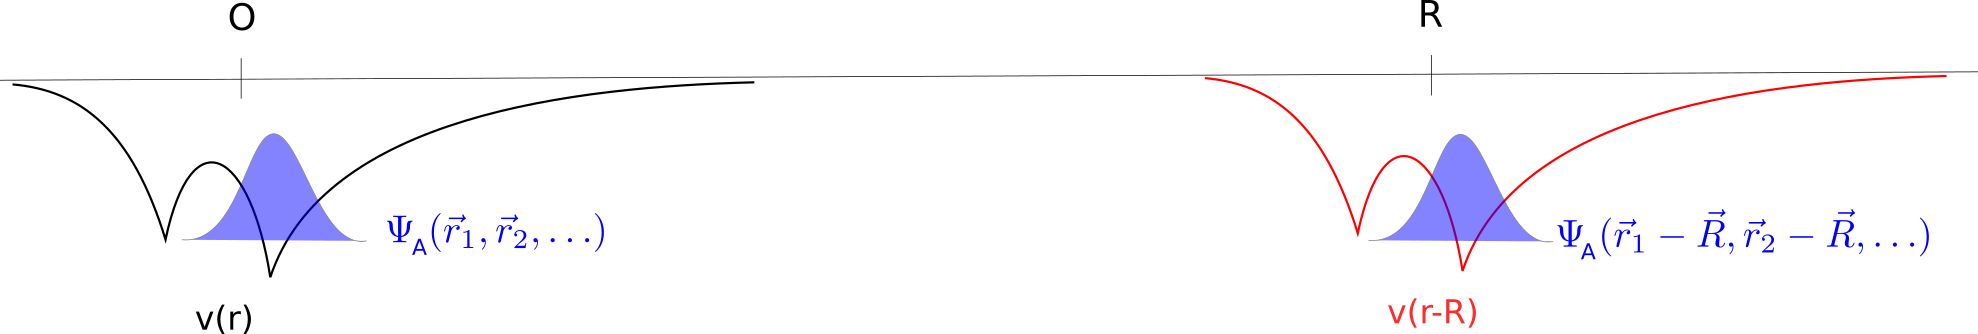
\includegraphics[width=0.9\linewidth]{figures/repeated_effective_potential.png}
  \caption{\label{fig:repeated_effective_potential} Effective potential of two identical molecules separated by a large distance $R$. The localized wavefunction in the left and right potential wells are identical except for the rigid shift.}
\end{figure}

$\mathbb{V}_{\vec{O}}^N$ is the subspace spanned by $N$ bound, electronic wavefunctions (not necessarily eigenstates) that are localized around the origin $\vec{O}$.
These wavefunctions decay exponentially with distance \cite{Katriel1980asymptotic}. $\mathbb{V}_{\vec{R}}^N$ is spanned by the same wavefunctions rigidly translated to the center $\vec{R}$. A subspace of twice the dimension is formed by combining the subspaces of the left and right molecules,
\begin{equation}
  \begin{split}
    \mathbb{V}^{2N} = \mathbb{V}^{N}_{\vec{O}} \cup \mathbb{V}^{N}_{\vec{R}} = \Span\Big\{ &
                  \Psi_1(\vec{r}_1,\vec{r}_2,\ldots),
                  \Psi_2(\vec{r}_1,\vec{r}_2,\ldots), \ldots,
                  \Psi_N(\vec{r}_1,\vec{r}_2,\ldots), \\
    &             \Psi_1(\vec{r}_1-\vec{R},\vec{r}_2-\vec{R},\ldots),
                  \Psi_2(\vec{r}_1-\vec{R},\vec{r}_2-\vec{R},\ldots), \ldots,
                  \Psi_N(\vec{r}_1-\vec{R},\vec{r}_2-\vec{R},\ldots) \Big\}.
  \end{split}
\end{equation}
Because of the large distance $R$, the transition densities between states localized at $\vec{O}$ and those at $\vec{R}$ vanish. The state densities and transition densities among the states localized on the same molecule are the same for both moleules except for a rigid shift. The matrix density for the combined subspace therefore consists of two blocks of size $N$, each:
\begin{equation}
  \m{D}^{(2N)}(\vec{r}) =
  \begin{pmatrix}
    \m{D}^{(N)}(\vec{r}) & 0 \\
    0 & \m{D}^{(N)}(\vec{r}-\vec{R})
  \end{pmatrix}
\end{equation}
As the distance between the two molecules is increased ($R \to \infty$), the matrix elements of the Hamiltonian vanishes, $\langle \Psi_{A} \vert \hat{H} \vert \Psi_{B} \rangle \to 0$, if the wavefunctions $\Psi_A$ and $\Psi_B$ are localized on different molecules. The matrix elements of the kinetic energy decrease exponentially, $\langle \Psi_{A} \vert \hat{T} \vert \Psi_{B} \rangle \propto \exp(-\alpha R)$, for the Coulomb operator the decrease is like $\langle \Psi_{A} \vert \hat{W} \vert \Psi_{B} \rangle \propto \frac{1}{R}$.
Therefore, in the limit $R \to \infty$, the universal part of the Hamiltonian in the subspace $\mathbb{V}^{(2 N)}$ is just block-diagonal, $\hat{H}^{(2N)}_0 = \hat{H}^{(N)} \oplus \hat{H}^{(N)}$. The projection of $\hat{H}_0$ into the combined subspace $\mathbb{V}^{(2N)}$ is a functional of the matrix density $\m{D}^{(2N)}$, and the Hamiltonians in the individual subspaces $\mathbb{V}^{(N)}_{\vec{O}}$ and $\mathbb{V}^{(N)}_{\vec{R}}$ are functionals of the matrix densities $\m{D}^{(N)}(\vec{r})$ and $\m{D}^{(N)}(\vec{r}-\vec{R})$, respectively. Furthermore the universal functional should be translationally invariant, so that $\m{\mathcal{F}}^{(N)}[\m{D}^{(N)}(\vec{r}-\vec{R})] = \m{\mathcal{F}}^{(N)}[\m{D}^{(N)}(\vec{r})] = \m{H}^{(N)}_0$. Therefore the following relation holds between the functionals $\m{\mathcal{F}}^{(2N)}$ and $\m{\mathcal{F}}^{(N)}$:
\begin{equation}
  \m{\mathcal{F}}^{(2N)}
  \left[
    \begin{pmatrix}
      \m{D}^{(N)}(\vec{r}) & 0 \\
      0 & \m{D}^{(N)}(\vec{r}-\vec{R})
    \end{pmatrix}
    \right]
  =
  \begin{pmatrix}
    \m{H}^{(N)}_{0} & 0 \\
    0 & \m{H}^{(N)}_{0}
  \end{pmatrix}
  =
  \begin{pmatrix}
    \m{\mathcal{F}}^{(N)}[\m{D}(\vec{r})] & 0 \\
    0 & \m{\mathcal{F}}^{(N)}[\m{D}(\vec{r})]
  \end{pmatrix} \label{eqn:relation_F2N_FN}
\end{equation}

The plan is to plug the functional Taylor expansion of Eqn.~\ref{eqn:functional_taylor_expansion} into Eqn.~\ref{eqn:relation_F2N_FN} in order to work out the relation between the functional $\m{\mathcal{F}}^{(2N)}$ and $\m{\mathcal{F}}^{(N)}$. A priori it is assumed that the functional could be different for different subspace dimensions. It will be shown that this is not the case. However, Eqn.~\ref{eqn:relation_F2N_FN} is not yet in a suitable form to compare the two functionals, since on its LHS the functional $\m{\mathcal{F}}^{(2N)}$ operates on a matrix density of dimension $2N$, while on the RHS the arguments of the functional $\m{\mathcal{F}}^{(N)}$ have dimension $N$. So we have to transform the expession in such a way, that $\m{\mathcal{F}}^{(2N)}$ operates on a matrix density of dimension $N$.
%%%

First some preliminaries.
The functional Taylor expansion involves integrations over three-dimensional space.
The three-dimensional space is partitioned into Voronoi polyhedra. Each point $\vec{r}$ is assigned to the closest molecule,
\begin{align}
  V_{\vec{O}} &= \{\vec{r}: \vert \vec{r} \vert < \vert \vec{r} - \vec{R} \vert \} \\
  V_{\vec{R}} &= \{\vec{r}: \vert \vec{r} - \vec{R} \vert \leq \vert \vec{r} \vert \} \\
  \mathbb{R}^3 &= V_{\vec{O}} \cup V_{\vec{R}}.
\end{align}
Integration over space is split into separate integrations over the Voronoi polyhedra,
\begin{equation}
 \int_{\mathbb{R}^3} \ldots d^3\!r = \int_{V_{\vec{O}}} \ldots d^3\!r + \int_{V_{\vec{R}}} \ldots d^3\!r.
\end{equation}
Since the wavefunctions are localized around the potential at either $\vec{O}$ or $\vec{R}$, there is no point in space where $\m{D}(\vec{r})$ and $\m{D}(\vec{r}-\vec{R})$ are simultaneously non-zero. So dependening on where the point $\vec{r}$ lies, the projection of the density operator in the subspace $\mathbb{V}^{2N}$ has only one non-zero block at the top or at the bottom:
\begin{equation}
  \m{D}^{(2N)}(\vec{r}) = \m{D}^{(N)}(\vec{r}) \oplus \m{D}^{(N)}(\vec{r}-\vec{R}) =
  \begin{cases}
    \m{D}^{(N)}(\vec{r}) \oplus 0 & \text{if } \vec{r} \in V_{\vec{O}} \\
    0 \oplus \m{D}^{(N)}(\vec{r}-\vec{R}) & \text{if } \vec{r} \in V_{\vec{R}} \label{eqn:D_split}
  \end{cases}
\end{equation}
Similarly we get for the trace,
\begin{equation}
  \tr\left(\m{D}^{(2N)}(\vec{r}) \right)
  =
  \tr\left(\m{D}^{(N)}(\vec{r}) \oplus \m{D}^{(N)}(\vec{r}-\vec{R}) \right)
  =
  \begin{cases}
    \tr(\m{D}(\vec{r})) & \text{if } \vec{r} \in V_{\vec{O}} \\
    \tr(\m{D}(\vec{r}-\vec{R}) & \text{if } \vec{r} \in V_{\vec{R}} \label{eqn:tr_split}
  \end{cases}
\end{equation}
If the functional should depend implicitly on the subspace dimension, the number of electronic states has to be expressed as a functional of the matrix density. One way to do this is
\begin{equation}
 \mathcal{N}(\vec{r}) = \tr\left\{ \m{D}(\vec{r}) \m{D}^{-1}(\vec{r}) \right\}.
\end{equation}
If at some point the matrix density does not have full rank and therefore is not invertible, the pseudinverse is used instead of the inverse. $\mathcal{N}(\vec{r})$ always equals the rank of the matrix density.
Since $\m{D}^{(2N)}(\vec{r})$ has at most rank $N$ (the number of wavefunctions that are simultaneously non-zero is at most $N$),
\begin{equation}
  \mathcal{N}^{(2N)}(\vec{r})
  =
  \begin{pmatrix}
    \mathcal{N}^{(N)}(\vec{r}) & \text{if } \vec{r} \in V_{\vec{O}} \\
    \mathcal{N}^{(N)}(\vec{r}-\vec{R}) & \text{if } \vec{r} \in V_{\vec{R}}. \label{eqn:N_split}
  \end{pmatrix}
\end{equation}

Now we write out the Taylor expansion and focus only on the term linear in $\m{D}^{(2N)}(\vec{r})$, but higher-order terms work the same way:

\begin{align}
  &\m{\mathcal{F}}^{(2N)}[\m{D}^{(2N)}(\vec{r})] = \int d^3\!r_1 ~ f^{(1)}\left(\vec{r}_1; \tr(\m{D}^{(2N)}(\vec{r}_1)), \mathcal{N}^{(2N)}(\vec{r}_1) \right) \m{D}^{(2N)}(\vec{r}_1) + \ldots \nonumber \\
    =& \int d^3\!r_1 ~ f^{(1)}\left(\vec{r}_1; \tr(\m{D}^{(2N)}(\vec{r}_1)), \mathcal{N}^{(2N)}(\vec{r}_1) \right)
    \begin{pmatrix}
      \m{D}^{(N)}(\vec{r}_1) & 0 \\
      0 & \m{D}^{(N)}(\vec{r}_1 - \vec{R})
    \end{pmatrix} + \ldots \nonumber \\
    =& \int_{V_{\vec{O}}} d^3\!r_1 ~ f^{(1)}\left(\vec{r}_1; \tr(\m{D}^{(N)}(\vec{r}_1)), \mathcal{N}^{(N)}(\vec{r}_1) \right)
    \begin{pmatrix}
      \m{D}^{(N)}(\vec{r}_1) & 0 \\
      0 & 0
    \end{pmatrix} \nonumber \\
    & + \int_{V_{\vec{R}}} d^3\!r_1 ~ f^{(1)}\left(\vec{r}_1; \tr(\m{D}^{(N)}(\vec{r}_1-\vec{R})), \mathcal{N}^{(N)}(\vec{r}_1-\vec{R}) \right)
    \begin{pmatrix}
      0 & 0 \\
      0 & \m{D}^{(N)}(\vec{r}_1-\vec{R})
    \end{pmatrix} + \ldots \nonumber \\
    =&
    \begin{pmatrix}
      \int_{\mathbb{R}^3} d^3\!r_1 ~ f^{(1)}\left(\vec{r}_1; \tr(\m{D}^{(N)}(\vec{r}_1)), \mathcal{N}^{(N)}(\vec{r}_1) \right) \m{D}^{(N)}(\vec{r}_1) + \ldots & 0 \\
      0 & \int_{\mathbb{R}^3} d^3\!r_1 ~ f^{(1)}\left(\ldots \right) \m{D}^{(N)}(\vec{r}_1-\vec{R}) + \ldots\\
    \end{pmatrix} \nonumber \\
    =&
    \begin{pmatrix}
      \m{\mathcal{F}}^{(2N)}[\m{D}^{(N)}(\vec{r})] & 0 \\
      0 & \m{\mathcal{F}}^{(2N)}[\m{D}^{(N)}(\vec{r})]
    \end{pmatrix} \label{eqn:relation_F2N_FN_same_dim}
\end{align}

In going from line 2 to 3 of Eqn.~\ref{eqn:relation_F2N_FN_same_dim}, the integration was split up and the corresponding cases from Eqns.~\ref{eqn:D_split},\ref{eqn:tr_split},\ref{eqn:N_split} were used inside each integration volume. In going from lines 3 and 4 to line 5, the integration range was extended again over the entire $\mathbb{R}^3$, since the respective integrands vanish on the additional volume. Finally, to get to the last line, we sum up the Taylor expansion again to obtain $\m{\mathcal{F}}^{(2N)}$ evaluated on the matrix density in the subspaces $\mathbb{V}_{\vec{O}}$ and $\mathbb{V}_{\vec{R}}$, respectively. As the universal functional has translational invariance, we can use $\m{\mathcal{F}}^{(2N)}[\m{D}^{(N)}(\vec{r}-\vec{R})] = \m{\mathcal{F}}^{(2N)}[\m{D}^{(N)}(\vec{r})]$.
Comparison of Eqn.~\ref{eqn:relation_F2N_FN_same_dim} with Eqn.~\ref{eqn:relation_F2N_FN} shows that
\begin{equation}
 \m{\mathcal{F}}^{(2N)}[\m{D}^{N}(\vec{r})] = \m{\mathcal{F}}^{(N)}[\m{D}^{N}(\vec{r})]
\end{equation}
for any matrix density $\m{D}^{(N)}(\vec{r})$ that decays exponentially with distance.


\section{Electron Repulsion}

\subsection{Correlation Functional}
\begin{figure}[h!]
  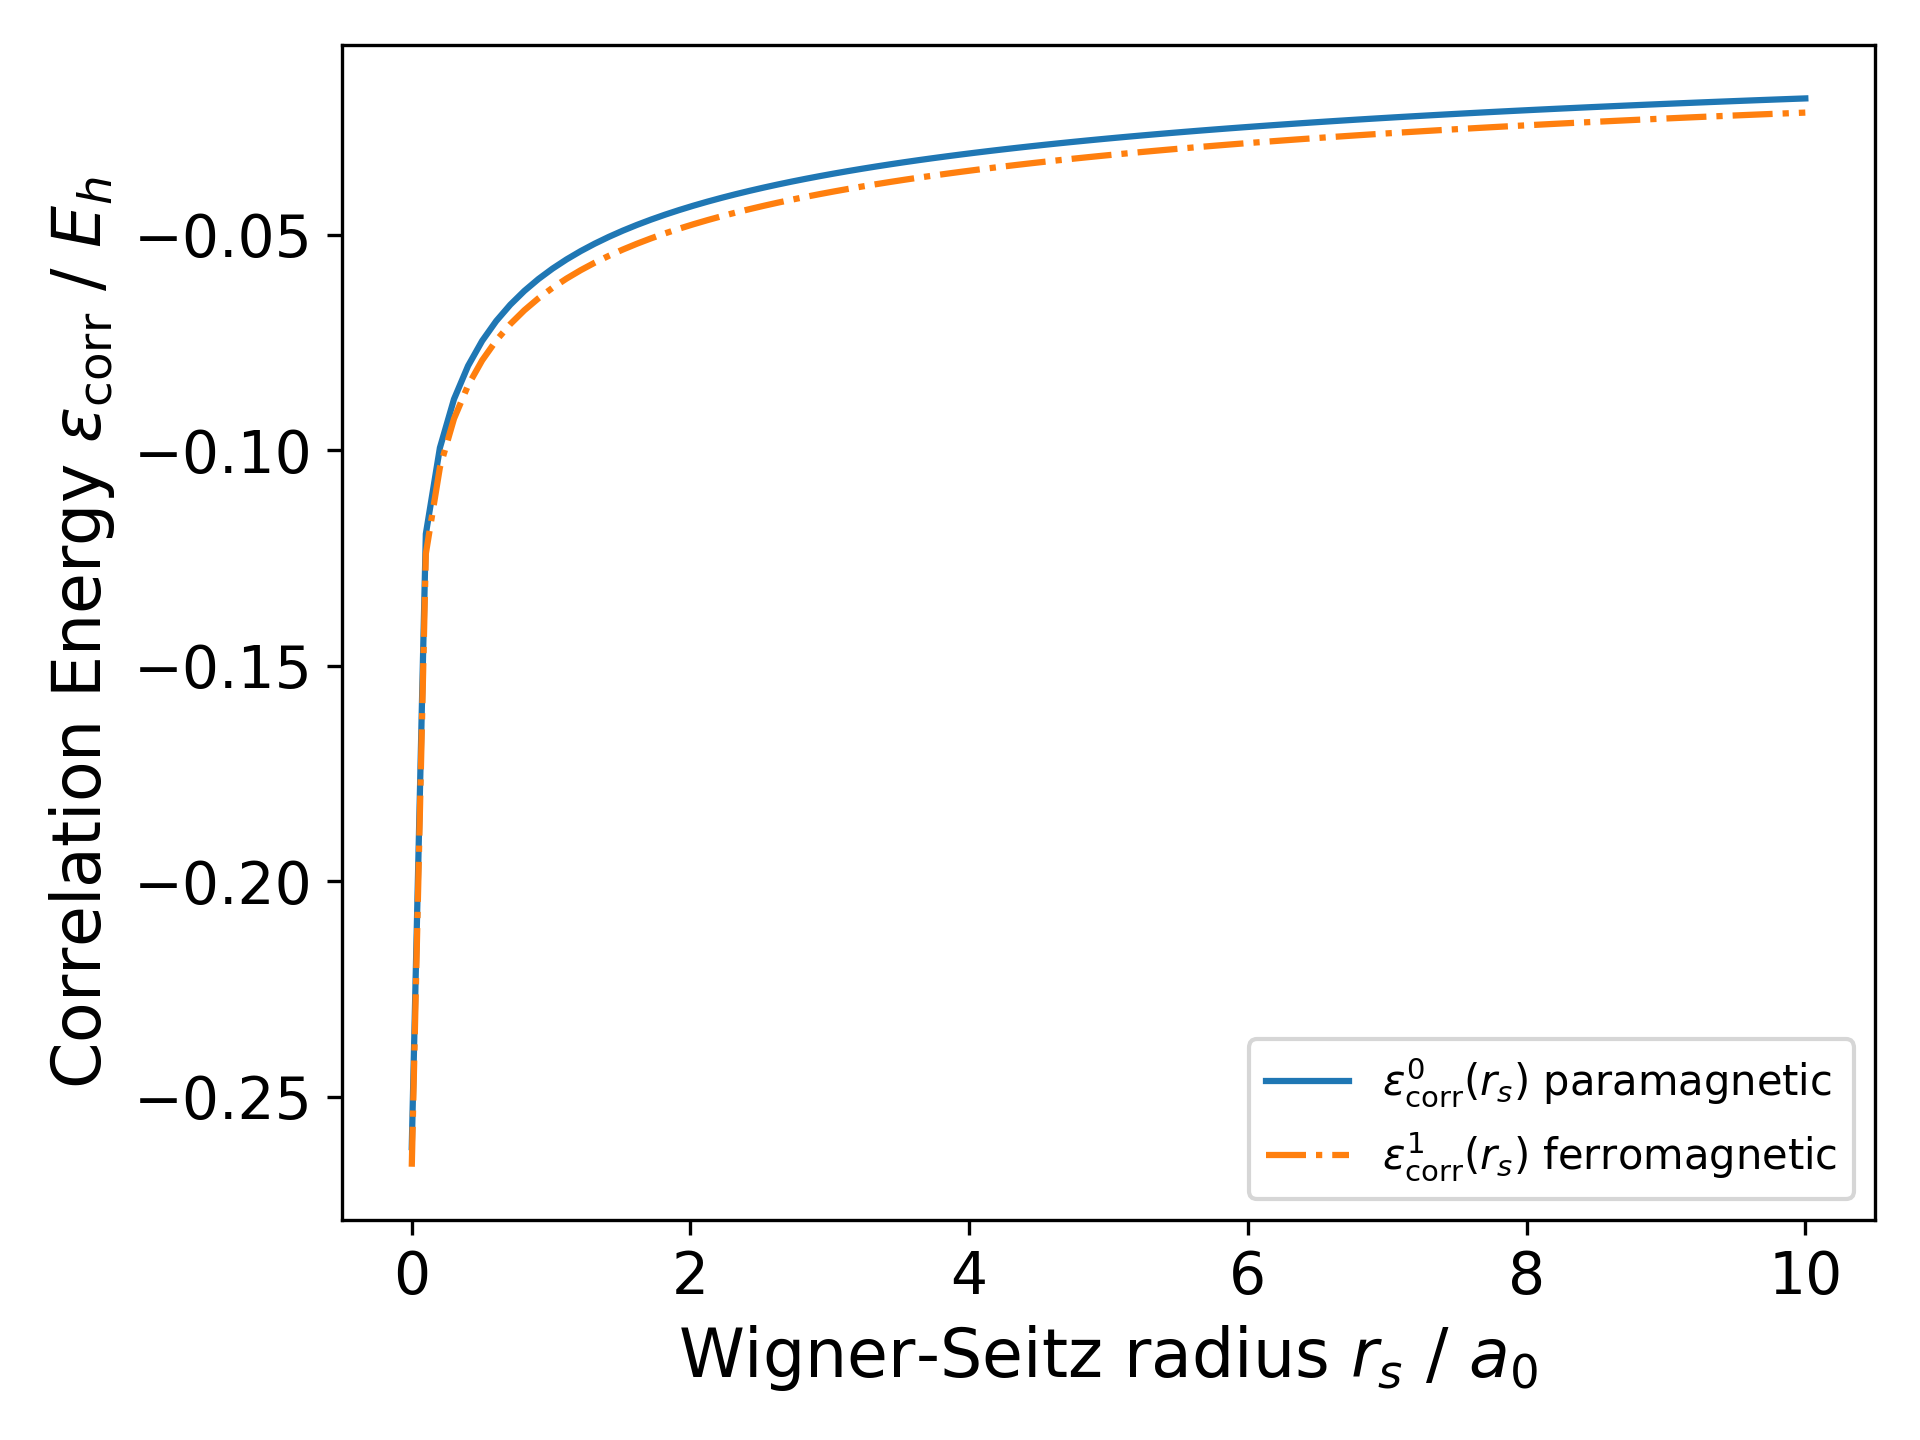
\includegraphics[width=0.5\linewidth]{figures/correlation_energy_paramagnetic_fs_ferromagnetic.png}
  \caption{\label{fig:correlation_energy_paramagnetic_fs_ferromagnetic}
  Paramagnetic (spin polarization $\zeta=0$) and ferromagnetic $\zeta=1$) correlation energy per particle
  $\epsilon_{\text{corr}}^{\zeta}$
  of a uniform electron gas with density $\rho = \frac{3}{4 \pi} r_s^{-3}$.
  The parameterization of Chachiyo \cite{Chachiyo2016} is used.}
\end{figure}
\FloatBarrier

\subsection{Klein's trace inequality}
\label{sec:Kleins_inequality}
Klein's inequality \cite{wiki:Kleins_inequality} \cite{Ruelle1969statistical} states that given two Hermitian, positive-definite $N \times N$ matrices $\m{A}$ and $\m{B}$ and
a convex function $f: \mathbb{R} \mapsto \mathbb{R}$ with derivative $f'$ the following trace inequality holds,
\begin{equation}
\tr\left[ f(\m{A}) - f(\m{B}) - (\m{A} - \m{B}) f'(\m{B}) \right] \ge 0 \label{eqn:Kleins_inequality}.
\end{equation}
With $f(x) = x^{4/3}$ (so that $f'(x) = 4/3 x^{1/3}$) and $\m{A} = \m{D}$ (full matrix) and $\m{B} = \Diag(\m{D}) = \Diag(D_{00}, D_{11}, \ldots, D_{NN})$ (only diagonal elements),
Klein's inequality becomes
\begin{equation}
\tr\left[ \m{D}^{4/3} - \Diag(\m{D})^{4/3} \right] \ge \tr\left[ \frac{4}{3} \left(\m{D} - \Diag(\m{D})\right) \Diag(\m{D})^{1/3}\right].
\end{equation}
The right hand side of this inequality is zero, since $\tr(\m{D} \Diag(\m{D})^{1/3}) = \tr(\Diag(\m{D})^{4/3})$, so that 
\begin{equation}
\tr(\m{D}^{4/3}(\vec{r})) \ge \sum_I D_{II}(\vec{r})^{4/3}.
\end{equation}
Integrating over space yields the inequality \ref{eqn:K_inequality}.

\section{Incorporating Exact Constraints}
\label{sec:exact_constraints}
Exact constraints can help to narrow down the form of a multistate functional.
This will be illustrated for the von-Weizs\"{a}cker functional.
The von-Weizs\"{a}cker functional $T[\rho]$ gives the exact kinetic energy for a single electron wavefunction $\phi(\vec{r}) = \sqrt{\rho(\vec{r})}$.
However, neither Eqn.~\ref{eqn:von_Weizsaecker_many_electrons} nor Eqn.~\ref{eqn:vW_ms_extension_matrix_square_root} yield the correct
matrix elements of the kinetic energy operator for a one-electron system.
In the following a kinetic energy functional is derived that reduces to the von-Weizs\"{a}cker functional for $N=1$ and gives the
exact kinetic energy matrix for single-electron wavefunctions.

Let the single particle wavefunctions be denoted as $\phi_I(\vec{r})$. With the help of Gauss' law
the matrix elements of the kinetic energy operator between states $I$ and $J$ can be expressed as
\begin{equation}
    T_{IJ} = -\frac{1}{2} \int d^3\!r ~ \phi^*_I \nabla^2 \phi_J
    = \int d^3\!r ~ \frac{1}{2} (\nabla \phi^*_I)\cdot (\nabla \phi_J). \label{eqn:kinetic_energy_1e}
\end{equation}
For a single-electron system, the matrix density is just the product of the wavefunctions (the density matrix),
\begin{equation}
 D_{IJ}(\vec{r}) = \phi^*_I(\vec{r}) \phi_J(\vec{r}).
\end{equation}
Note that for wavefunctions of a single electron
\begin{equation}
 \sum_{K=1}^{N} D_{IK} D_{KJ} = \phi^*_I \sum_{K} \phi_{K} \phi^*_{K} \phi_J = \tr(\m{D}) D_{IJ},
\end{equation}
however, this relation is not true for matrix densities of multi-electron systems.

To derive the von-Weizs\"{a}cker kinetic energy functional one has to assume that all wavefunctions are real, so that $D_{IJ} = \phi_I \phi_J$.
Now consider
\begin{equation}
\begin{split}
  & \sum_K (\nabla D_{IK}) \cdot (\nabla D_{KJ})
  = \sum_K (\nabla \phi_I \phi_K + \phi_I \nabla \phi_K)\cdot (\nabla \phi_K \phi_J + \phi_K \nabla \phi_J) \\
  =&
  (\sum_K \phi_K \phi_K) \nabla \phi_I \cdot \nabla \phi_J +
  \sum_K (\nabla \phi_K \cdot \nabla \phi_K) \phi_I \phi_J +
  \sum_K (\nabla \phi_I \cdot \nabla \phi_K) \phi_K \phi_J +
  \sum_K \phi_I \phi_K (\nabla \phi_K \cdot  \nabla \phi_J) \\
  =& \tr(\m{D}) (\nabla \phi_I \cdot \nabla \phi_J) + D_{IJ} \sum_{K} (\nabla \phi_K \cdot \nabla \phi_K) + \sum_K (\nabla \phi_I \cdot \nabla \phi_K) D_{KJ}
  + \sum_K D_{IK} (\nabla \phi_K \cdot \nabla \phi_J)
\end{split}
\end{equation}
The kinetic energy density $T_{IJ}(\vec{r}) = \frac{1}{2} \nabla \phi_I(\vec{r}) \cdot \nabla \phi_J(\vec{r})$ (the integrand in Eqn.~\ref{eqn:kinetic_energy_1e}) appears on the right hand side multiple times. Rewriting the previous equation in terms of $T_{IJ}(\vec{r})$ gives
\begin{equation}
T_{IJ}(\vec{r}) = \underbrace{\frac{1}{2} \frac{\sum_K \nabla D_{IK} \cdot \nabla D_{KJ}}{\tr(\m{D})}}_{C_{IJ}(\vec{r})} - \underbrace{\frac{D_{IJ}}{\tr(\m{D})}}_{R_{IJ}(\vec{r})} \sum_K T_{KK}(\vec{r}) - \sum_{K} T_{IK}(\vec{r}) \underbrace{\frac{D_{KJ}}{\tr(\m{D})}}_{R_{KJ}(\vec{r})} - \sum_{K} \underbrace{\frac{D_{IK}}{\tr(\m{D})}}_{R_{IK}(\vec{r})} T_{KJ}(\vec{r}) \label{eqn:kinetic_density_multistate}
\end{equation}
For a single electronic state ($N=1$), we get $C = \frac{1}{2} (\nabla \rho)\cdot (\nabla \rho) / \rho$, $R = 1$ and the above equation reduces to
\begin{equation}
t_{\text{vW}}(\vec{r}) = \frac{1}{2} \frac{\nabla \rho \cdot \nabla \rho}{\rho} - 3 t_W(\vec{r})
\end{equation}
or
\begin{equation}
t_{\text{vW}}(\vec{r}) = \frac{1}{8} \frac{\nabla \rho(\vec{r}) \cdot \nabla \rho(\vec{r})}{\rho(\vec{r})}, \label{eqn:von_Weizsaecker_ked}
\end{equation}
which is the kinetic energy density of the familiar von-Weizs\"{a}cker functional \cite{Weizsacker1935},
\begin{equation}
  T_{\text{vW}}[\rho] = \int t_{\text{vW}}[\rho](\vec{r}) d^3\!r  \label{eqn:von_Weizsaecker_functional}.
\end{equation}
For $N > 1$ Eqn.~\ref{eqn:kinetic_density_multistate} is a system of linear equations,
\begin{equation}
 T_{IJ}(\vec{r}) = C_{IJ} - R_{IJ} \sum_K T_{KK} - \sum_K T_{IK} R_{KJ} - \sum_K R_{IK} T_{KJ}
\end{equation}
that has to be solved for $T_{IJ}(\vec{r})$ at each point $\vec{r}$.
To solve the linear system, $T_{IJ}(\vec{r})$ is treated as a vector in $\mathbb{R}^{N \times N}$ and the equation is rewritten as
\begin{equation}
T_{IJ}(\vec{r}) = C_{IJ}(\vec{r}) + \sum_{K,L=1}^{N} \mathcal{K}_{IJ,KL}(\vec{r}) T_{KL}(\vec{r}) \label{eqn:CplusKT}
\end{equation}
This equation has the form $\vec{T} = \vec{C} + \mathcal{K} \vec{T}$, which can be solved for the vector $\vec{T} = (1 - \mathcal{K})^{-1} \vec{C}$.
By writing Eqn.~\ref{eqn:CplusKT} as
\begin{equation}
T_{IJ}(\vec{r}) = C_{IJ}(\vec{r}) + \sum_{K,L} \left\{ - R_{IK}(\vec{r}) \delta_{LJ} - \delta_{IK} R_{LJ}(\vec{r}) - R_{IJ}(\vec{r}) \delta_{KL} \right\} \vec{T}_{KL}(\vec{r}) \label{eqn:vonWZ_matrix_equation}
\end{equation}
we see that the matrix $\mathcal{K} \in \mathbb{R}^{N^2 \times N^2}$ is
\begin{equation}
 \mathcal{K}_{IJ,KL} = - R_{IK}(\vec{r}) \delta_{LJ} - \delta_{IK} R_{LJ}(\vec{r}) - R_{IJ}(\vec{r}) \delta_{KL}
\end{equation}
Under the assumption $\lvert \mathcal{K} \rvert < 1$, $(1 - \mathcal{K})^{-1}$ can be written as a geometric series
\begin{equation}
 (1 - \mathcal{K})^{-1} = \sum_{k=0}^{\infty} \mathcal{K}^{k}
\end{equation}
so that
\begin{equation}
\vec{T} = \sum_{k=0}^{\infty} \mathcal{K}^{k} \vec{C} = \vec{C} + \sum_{k=1}^{\infty} \mathcal{K}^{k} \vec{C} \label{eqn:solution_geometric_series}
\end{equation}
To prove $\lvert \mathcal{K} \rvert < 1$, we have to show that $R_{IJ} < 1$. This follows from
\begin{equation}
D_{IJ}(\vec{r}) = \phi_I(\vec{r}) \phi_J(\vec{r}) \leq \max_{K} \phi_K(\vec{r}) \phi_K(\vec{r}) \leq \sum_K \phi_K(\vec{r}) \phi_K(\vec{r}) = \tr(\m{D})
\end{equation}
Eqn.~\ref{eqn:solution_geometric_series} demonstrates that the kinetic energy density obtained by solving Eqn.~\ref{eqn:vonWZ_matrix_equation} is indeed a functional of the matrix density $\m{D}$. The first term of the series \ref{eqn:solution_geometric_series} is
\begin{equation}
\begin{split}
  (\mathcal{K} \vec{C})_{IJ} &= -\sum_{K} R_{IK} C_{KJ} - \sum_{K} C_{IK} R_{KJ} - R_{IJ} \sum_K C_{KK} \\
   &= - (\m{R} \m{C} + \m{C} \m{R})_{IJ} - R_{IJ} \tr(\m{C}).
\end{split}
\end{equation}
Since $\m{R}$ and $\m{C}$ are analytic matrix functionals of $\m{D}$, i.e. $\m{R}[\m{U} \m{D} \m{U}^{-1}] = \m{U} \m{R}[\m{D}] \m{U}^{-1}$ and similarly for $\m{C}$,
we conclude that $\mathcal{K} \vec{C}$ and $\mathcal{K} (\mathcal{K} \vec{C})$ etc. are analytic matrix functionals, which only depend on $\m{D}(\vec{r})$, $\nabla \m{D}(\vec{r})$ and the scalar invariant $\tr(\m{D})$, as well.

Although for $N=1$ it reduces to the simple expression in Eqn.~\ref{eqn:von_Weizsaecker_functional},
the \emph{multistate} von-Weizsaecker functional of Eqn.~\ref{eqn:solution_geometric_series} is an infinite series. 
This suggests that trying to guess the functional form of a matrix density functional from a known ground state functional
with non-commuting terms (such as functionals from the generalized gradient approximation (GGA) family)
will in general not be crowned with success.
Taking only the first two terms of the infinite series, the kinetic energy functional reads
\begin{equation}
\begin{split}
  \m{T}_{\text{vW1e}}[\m{D}(\vec{r})] =& \int \m{C} ~ d^3\!r  - \int \left(\m{R} \m{C} + \m{C} \m{R} + \tr(\m{C}) \m{R} \right) d^3\!r  + \ldots \\
  =& \int \frac{1}{2} \tr(\m{D})^{-1} (\nabla \m{D} \cdot \nabla \m{D}) ~ d^3\!r \\
  & - \int \frac{1}{2} \tr(\m{D})^{-2} \left[ \m{D} (\nabla \m{D} \cdot \nabla \m{D}) + (\nabla \m{D} \cdot \nabla \m{D}) \m{D} + \tr(\nabla \m{D} \cdot \nabla \m{D}) \m{D} \right] ~ d^3\!r + \ldots .
\end{split}
\label{eqn:TvW1e}
\end{equation}
In practice $\m{T}_{\text{vW1e}}[\m{D}(\vec{r})]$ is determined by solving Eqn.~\ref{eqn:CplusKT} for
each grid point and then integrating the kinetic energy density numerically.

Figures \ref{fig:vW_kinetic_energy_HMI} and \ref{fig:vW_kinetic_energy_LiH} compare the kinetic energy densities
of two von-Weizs\"{a}cker-like functionals $\m{T}_{\text{vW}}$ (Eqn.~\ref{eqn:von_Weizsaecker_many_electrons})
and $\m{T}_{\text{vW1e}}$ (Eqn.~\ref{eqn:TvW1e}) with the exact results
computed with full configuration interaction as implemented in the PySCF \cite{Sun2020} software package. Clearly \textbf{vW1e} is exact for 1-electron systems
but significantly understimates the kinetic energy density for multiple electrons.
The \textbf{vW} functional works well in the vicinity of the nuclei where the electron density is high, but less so in the bonding regions.
But both functionals reproduce the transition density accurately.
More exact conditions are needed to constrain the kinetic energy functional.
%Reproducing the exact kinetic energy matrix on density matrices belonging to one-particle wavefunctions is not 

\begin{figure}[h!]
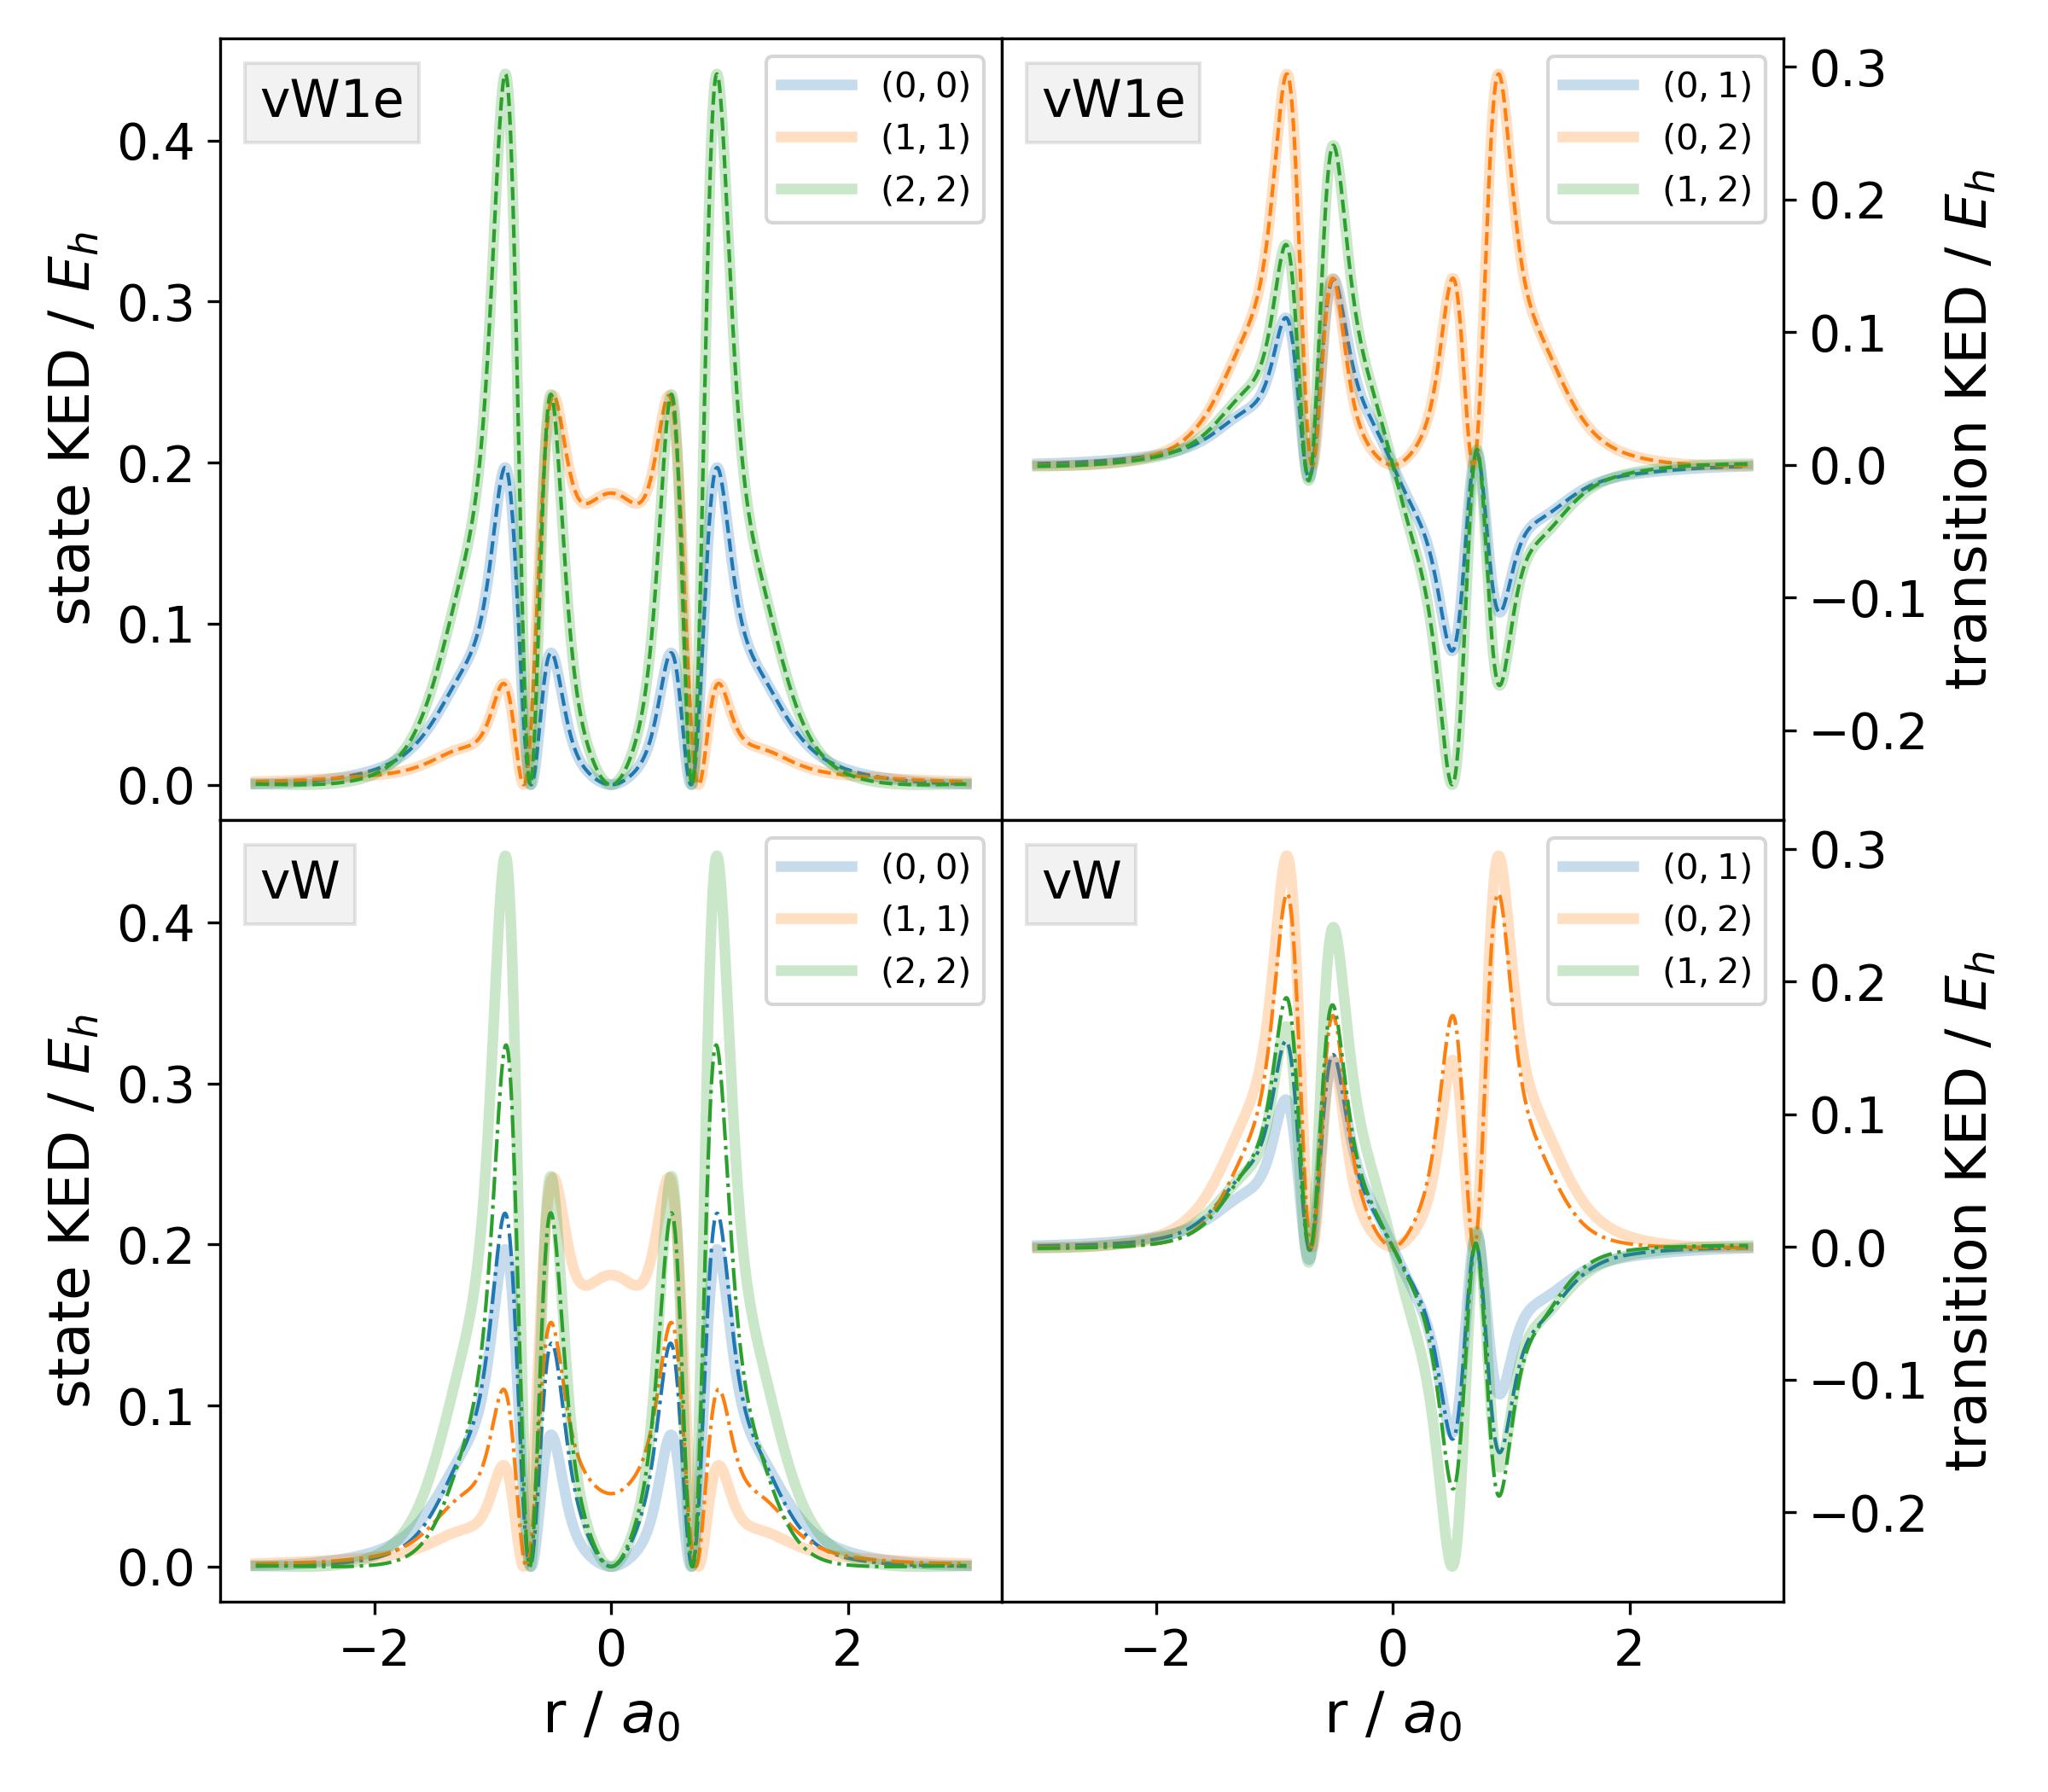
\includegraphics[width=0.8\textwidth]{figures/vW_kinetic_energy_HMI.png}
\caption{\textbf{1-electron system.} Cut through the kinetic energy density (KED) of hydrogen molecular ion, H$_2^+$, along the bond axis for the lowest three electronic states $I,J=0,1,2$. Solid, thick lines represent the exact kinetic energy density computed as ${T_{IJ} = -\frac{1}{2} \int \nabla \phi_I(\vec{r}) \cdot \nabla \phi_J(\vec{r})}$ from a calculation with the 6-31g basis set using PySCF. Dashed, thin lines are the KEDs computed with approximate kinetic energy functionals according to Eqn.~\ref{eqn:solution_geometric_series} (\textbf{vW1e}) and Eqn.~\ref{eqn:von_Weizsaecker_many_electrons} (\textbf{vW}). Diagonal state KED's $(I,I)$ are shown on the left, transition KED's $(I,J)$ on the right.}
\label{fig:vW_kinetic_energy_HMI}
\end{figure}

\begin{figure}[h!]
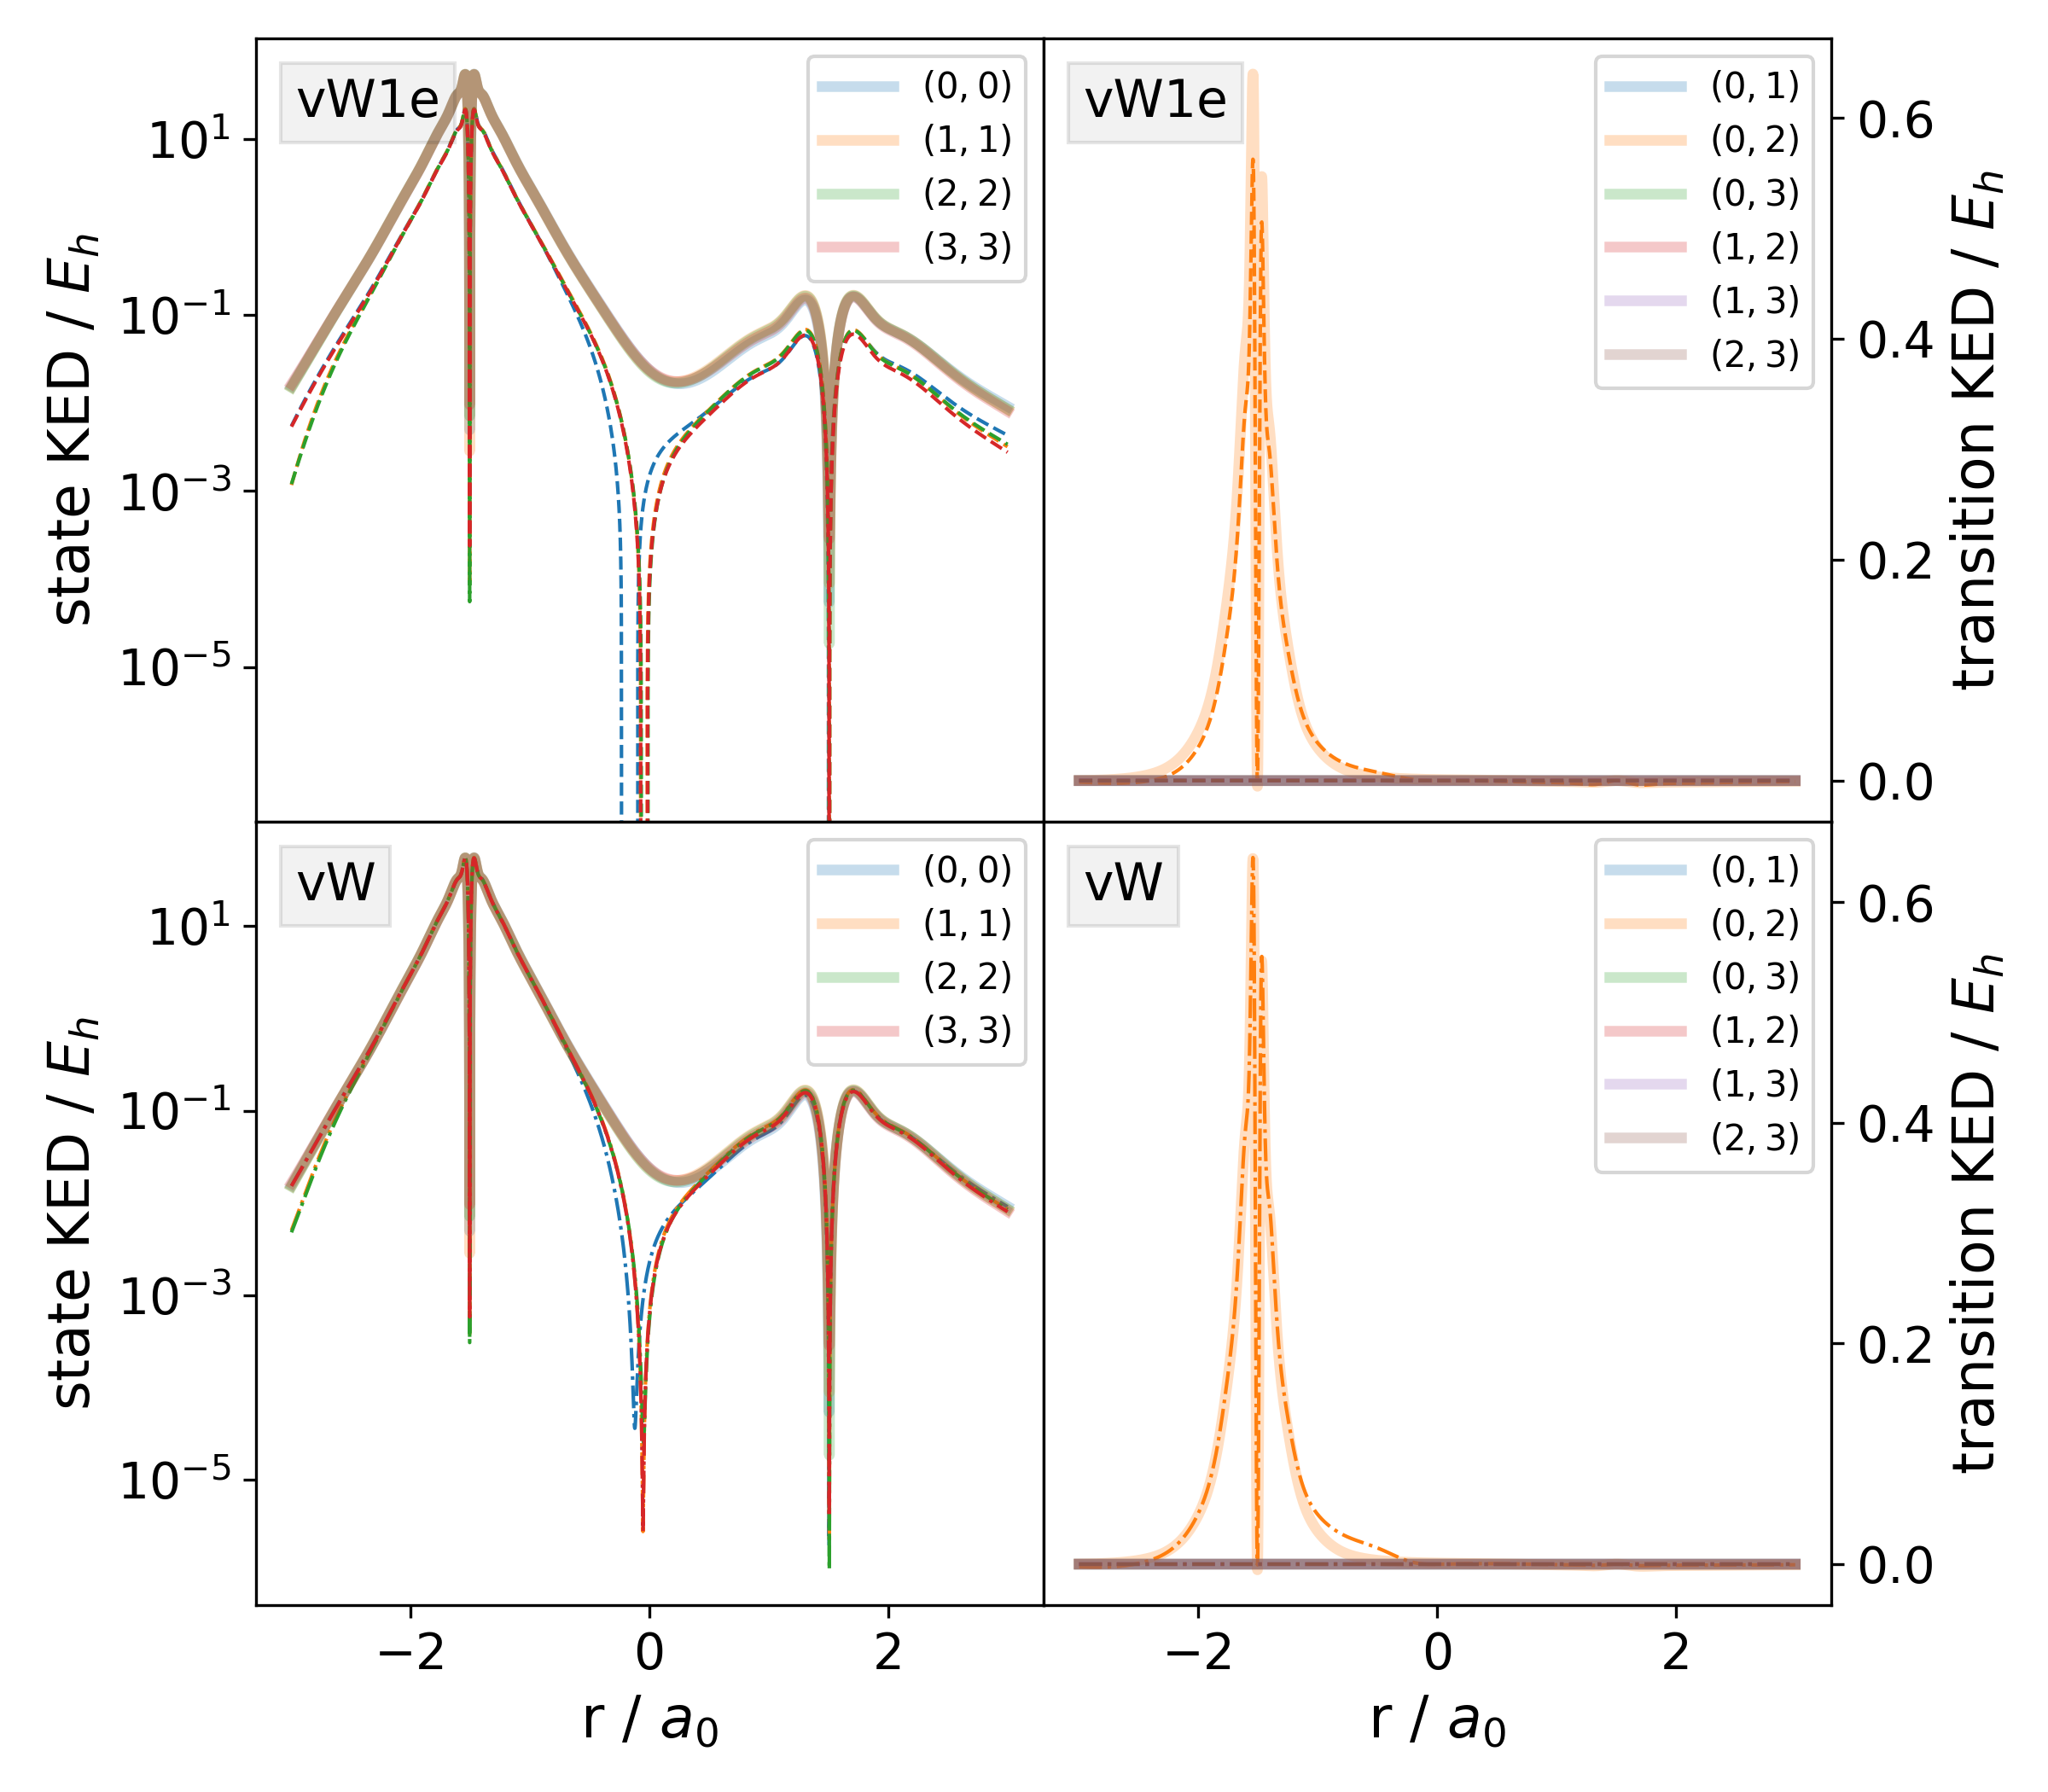
\includegraphics[width=0.8\textwidth]{figures/vW_kinetic_energy_LiH-lda.png}
\caption{\textbf{Lithium hydride.} Cut through the kinetic energy density (KED) of lithium hydride, LiH, along the bond axis for the lowest four electronic states $I,J=0,1,2,3$. Solid, thick lines represent the exact kinetic energy density from a FCI/6-31g calculation using PySCF. Dashed, thin lines are the KEDs computed with approximate kinetic energy functionals according to Eqn.~\ref{eqn:solution_geometric_series} (\textbf{vW1e}) and Eqn.~\ref{eqn:von_Weizsaecker_many_electrons} (\textbf{vW}). Diagonal state KED's $(I,I)$ are shown on the left (log), transition KED's $(I,J)$ on the right.}
\label{fig:vW_kinetic_energy_LiH}
\end{figure}

\FloatBarrier

\section{Excited States of the Homogeneous Electron Gas}
\label{sec:heg_msdft}
Except for the von-Weizs\"{a}cker correction all multistate functionals presented above are local density approximations.
The LDA expressions are derived from the homogeneous electron gas, where the density is a constant,
and are transferred to inhomogeneous systems.
Assuming that the density changes little within a small volume element $d^3\!r$,
the homogeneous electron gas expressions are applied to the density in each volume element. Summing
over all space gives the total energy. The LDA is exact for the ground state of the homogeneous electron gas,
but what about the multistate version of LDA? Is it exact for the excited states of the homogeneous electron gas?
And how do the lowest excited state of the homogeneous electron gas look like?

In order to maintain the validity of the LDA, the excited state wavefunctions have to be constants, too.
One can construct a homogeneous wavefunction with higher kinetic energy than the ground state by removing electrons
below the Fermi level and putting them into plane wave states above the Fermi level. \cite{Hemanadhan2010}
However, no matter how the electrons are distributed in k-space, the electron density will not change
since $\vert e^{\imath \vec{k} \cdot \vec{r}} \vert = 1$ for any $\vec{\vec{k}}$.
Therefore the diagonal elements of the matrix density are the same constant $D_{II}(\vec{r}) = \rho = \frac{n}{V}$
(number of electrons $n$ per volume $V$) for all states $I$.
However, the states become distinguishable when the transition densities are taken into account.
The transition densities are non-zero only between states that differ at most in the occupation of two plane-wave orbitals.
Let us assume that in the transition from the state $I$ to $J$, the wave vector of one electron is changed from
$\vec{k}_I$ to $\vec{k}_J$. Then the transition density is
$D_{IJ}(\vec{r}) = \frac{1}{\sqrt{V}} e^{\imath (\vec{k}_J - \vec{k}_I) \cdot \vec{r}}$.
However, there is a problem. The homogeneous electron gas does not have a gap between the ground state and the first excited state.
Also, since the homogeneous electron gas is of infinite size, the states form a continuum. Of course, one could pick out a subspace of $N$
electronic states and construct the matrix density. 
However, the matrix functional gives the exact Hamiltonian matrix only for the lowest $N$ electronic states.
For a random set of electronic states there is no guarantee that $\m{F}[\m{D}] + \int v(\vec{r}) \m{D}(\vec{r}) ~ d^3\!r$
maps their matrix density to the corresponding Hamiltonian matrix.
The only thing we know is that the average energy of those states will be larger than the average energy
of the same number of lowest-energy states. For a continuous spectrum the variational minimization of the subspace energy is not possible.
These considerations suggest that MSDFT is only applicable to bounds states of finite systems, which have a discrete spectrum
so that a matrix representation is adequate.


\section{Lower Bounds}
\label{sec:lower_bounds}
When searching for approximate density functionals, lower bounds on the kinetic energy and the exchange-correlation energy
are very useful. In the multistate density functional theory, the subspace expectation value of the energy is minimized
(Eqn.~(13) in Ref.~\cite{Lu2022JPCL}), which is the state-averaged (or MS for \emph{multistate}) energy,
\begin{equation}
  E_{\text{MS}}[\m{D}] = \frac{1}{N} \sum_{I=1}^{N} \mathcal{H}_{II}[\m{D}]
  = \frac{1}{N} \sum_{I=1}^{N} \left( \m{\mathcal{F}}_{II}[\m{D}] + \int d^3r ~ v(\vec{r}) D_{II}(\vec{r}) \right).
\end{equation}
Therefore one has to bound $\frac{1}{N} \tr(\m{\mathcal{F}}[\m{D}])$ from below rather than finding bounds of
the individual matrix elements $\mathcal{F}_{IJ}[\m{D}]$. The lower bounds for the average kinetic and electron repulsion energies
will be treated separately.

\subsubsection{Lower Bound of Kinetic Energy}
The kinetic energy of a single wavefunction is bounded from below by the von-Weiz\"{a}cker kinetic energy functional.
The proof for this inequality can be found below theorem 1.1 of Ref.~\cite{Lieb2002}. Applying this bound individually
to each electronic state in the subspace and averaging over states, one obtains a lower bound on the subspace kinetic energy,
\begin{equation}
 \frac{1}{N} \sum_{I=1}^{N} T_{II} \ge \frac{1}{N} \int d^3r ~ \frac{1}{8} \sum_{I=1}^{N} \frac{\vert \nabla D_{II}(\vec{r}) \vert^2}{D_{II}(\vec{r})}.
 \label{eqn:lower_bound_kinetic_sum_over_states}
\end{equation}
However, while the left hand side is a subspace invariant, i.e. it does not change under a basis transformation of the vectors in the subspace,
the right hand side is not. It is possible to find a bound on the average kinetic energy that is almost as tight but also is a subspace invariant.
The derivation proceeds in analogy with theorem 1.1 of Ref.~\cite{Lieb2002}. It is assumed that the $n$-electron wavefunctions are antisymmetric and orthonormal.
The wavefunctions in the subspace are put into an $N$-dimensional vector
$\vec{\Psi}(\vec{x}_1,\ldots,\vec{x}_n) = \left(\Psi_1(\vec{x}_1,\ldots,\vec{x}_n), \ldots, \Psi_N(\vec{x}_1,\ldots,\vec{x}_n)\right)$. One then defines
a scalar product on this vector space,
\begin{equation}
\langle \vec{\Psi}, \vec{\Phi} \rangle({\color{red} \vec{r}_1}) = \sum_{I=1}^{N} \sum_{\sigma_1=\uparrow,\downarrow} \int dx_2 \int dx_3 \cdots \int dx_n
  \Psi_I^*({\color{red} \vec{r}_1},\sigma_1;\vec{x}_2,\ldots,\vec{x}_n)
  \Phi_I({\color{red} \vec{r}_1},\sigma_1;\vec{x}_2,\ldots,\vec{x}_n),
\end{equation}
which sums over all electronic states $I=1,\ldots,N$ and integrates over all spatial and spin coordinates $\vec{x}_i = (\vec{r}_i,\sigma_i)$ for $i=2,\ldots,n$
except for the spatial coordinates ${\color{red} \vec{r}_1}$
of the first electron. The scalar product is therefore a function of $\vec{r}_1$. The integral over all coordinates except for $\vec{r}_1$ is abbreviated
by the symbol $\int^{\dagger} \ldots := \sum_{\sigma_1=\uparrow,\downarrow} \int dx_2 \int dx_3 \cdots \int dx_n \ldots$ ~.
Since the electrons are indistinguishable, it does not matter which electronic coordinate is left out in the integral.
The remaining electronic coordinate is denoted by $\vec{r} = \vec{r}_1$.
Since $\langle \vec{\Psi},\vec{\Psi} \rangle = n \sum_{I} D_{II}(\vec{r})$,
the gradient of the sum of the electron densities with respect to the remaining electron coordinate can be expressed as a scalar product,
\begin{equation}
  \begin{split}
 \sum_I \nabla D_{II}(\vec{r}) &= n \sum_I \int^{\dagger} \nabla \Psi_I^* \Psi_I + n \sum_I \int^{\dagger} \Psi_I^* \nabla \Psi_I \\
  &= n \langle \nabla \vec{\Psi}, \vec{\Psi} \rangle + n \langle \vec{\Psi}, \nabla \vec{\Psi} \rangle, \\
  \end{split}
\end{equation}
which is bounded from above by the triangle inequality,
\begin{equation}
  \begin{split}
\left\vert \sum_I \nabla D_{II}(\vec{r}) \right\vert &=
\left\vert n \langle \nabla \vec{\Psi}, \vec{\Psi} \rangle + n \langle \vec{\Psi}, \nabla \vec{\Psi} \rangle \right\vert \\
& \leq n \vert \langle \nabla \vec{\Psi}, \vec{\Psi} \rangle \vert + n \vert \langle \vec{\Psi}, \nabla \vec{\Psi} \rangle \vert \\
&= 2 n \vert \langle \nabla \vec{\Psi}, \vec{\Psi} \rangle \vert. \label{eqn:triangle_inequality}
  \end{split}
\end{equation}
$\vert \langle \nabla \vec{\Psi}, \vec{\Psi} \rangle \vert$ is bounded by the Cauchy-Schwarz inequality,
\begin{equation}
  \begin{split}
  \vert \langle \nabla \vec{\Psi}, \vec{\Psi} \rangle \vert^2 &\leq
  \vert \langle \nabla \vec{\Psi}, \nabla \vec{\Psi} \rangle \vert \vert \langle \vec{\Psi}, \vec{\Psi} \rangle \vert \\
  &= \sum_I \int^{\dagger} \vert \nabla \Psi_I \vert^2 ~ \frac{1}{n} \sum_{J} D_{JJ}. \label{eqn:Cauchy_Schwarz}
  \end{split}
\end{equation}
In $n \int^{\dagger} \frac{1}{2} \vert \nabla \Psi_I \vert^2$ one recognizes the kinetic energy density $T_{II}(\vec{r})$ of the electronic state $I$.
Combining the inequalities \ref{eqn:triangle_inequality} and \ref{eqn:Cauchy_Schwarz} one gets
\begin{equation}
  \begin{split}
 \vert \sum_I \nabla D_{II}(\vec{r}) \vert^2 &\leq 4 n^2 \left(\sum_I \int^{\dagger} \vert \nabla \Psi_I \vert^2 \right) \left( \frac{1}{n} \sum_J D_{JJ} \right) \\
 &= 8 \left( \sum_I n \int^{\dagger} \frac{1}{2} \vert \nabla \Psi_I \vert^2 \right) \sum_J D_{JJ} \\
 &= 8 \sum_I T_{II}(\vec{r}) \sum_J D_{JJ}(\vec{r}),
  \end{split}
\end{equation}
which can be rearranged into
\begin{equation}
 \sum_I T_{II}(\vec{r}) \geq \frac{1}{8} \frac{\vert \sum_I \nabla D_{II}(\vec{r}) \vert^2}{\sum_J D_{JJ}(\vec{r})}.
\end{equation}
This inequality holds at very point in space. Dividing both sides by the number of states, expressing the right hand side in terms of the subspace
density $\rho_{V} = \frac{1}{N} \tr(\m{D}) = \frac{1}{N} \sum_I D_{II}(\vec{r})$, and integrating over the remaining electron coordinate,
the lower bound on the average kinetic energy of the subspace becomes
\begin{equation}
\frac{1}{N} \sum_{I=1}^{N} \langle \Psi_I \vert \sum_{i=1}^{n} \left(-\frac{1}{2} \nabla_i^2 \right) \vert \Psi_I \rangle
\geq \frac{1}{8} \int \frac{\left\vert \nabla \rho_{V}(\vec{r}) \right\vert^2}{\rho_{V}(\vec{r})} d^3r.
\label{eqn:lower_bound_kinetic_subspace_invariant}
\end{equation}
This lower bound is a functional of the subspace density $\rho_{V}(\vec{r})$ and is therefore an invariant property of the subspace.
Table \ref{tbl:lower_bounds_kinetic_energy} compares the exact average kinetic energy of the lowest 4 states for a few small molecules
with the lower bounds according to Eqn.~\ref{eqn:lower_bound_kinetic_sum_over_states}
and Eqn.~\ref{eqn:lower_bound_kinetic_subspace_invariant}, respectively.
For one-electron systems the bound of Eqn.~\ref{eqn:lower_bound_kinetic_sum_over_states} is exact. For molecules with many electrons,
both bounds are very close to each other, with the invariant bound of Eqn.~\ref{eqn:lower_bound_kinetic_subspace_invariant} slightly
less tight than that of Eqn.~\ref{eqn:lower_bound_kinetic_sum_over_states}. Overall the bounds are not tight enough to be very useful.


%%%%%%%%%%%%%%%%%%%%%% AUTO-GENERATE LATEX CODE (format_latex_table.py) %%%%%%%%%%%%%%%%%%%%%%%%%%%%%%%%%%%%%%%
\sisetup{
round-mode = places,
round-precision = 3,
scientific-notation = fixed,
fixed-exponent = 0,
zero-decimal-to-integer
}

\begin{table}
\begin{tabular}{
  SSSSS
  }
    \toprule
 {Molecule} & {Basis} & {Bound Eqn.~\ref{eqn:lower_bound_kinetic_Lieb}} & {Bound Eqn.~\ref{eqn:lower_bound_kinetic_invariant}} & {Exact}\\
\midrule
{H} & {6-31g} & 1.143235 & 0.823160 & 1.143235 \\
{H (large basis set)} & {aug-cc-pvtz} & 0.292371 & 0.150067 & 0.292371 \\
{H$_2^+$} & {6-31g} & 1.250525 & 0.767747 & 1.250525 \\
{H$_2$} & {6-31g} & 1.146228 & 0.973287 & 1.434804 \\
{Li} & {6-31g} & 7.206488 & 7.146008 & 7.384005 \\
{LiH} & {6-31g} & 7.669143 & 7.613865 & 7.976373 \\
{water} & {sto-3g} & 57.577183 & 57.446115 & 75.553086 \\
{O$_2$} & {sto-3g} & 113.211488 & 113.163189 & 146.582754 \\
{NO} & {sto-3g} & 99.286293 & 99.202325 & 126.551376 \\
{He} & {6-31g} & 4.157342 & 3.462193 & 4.649976 \\
{Ne} & {6-31g} & 90.150973 & 90.096788 & 130.121379 \\
\bottomrule
\end{tabular}

\caption{
\label{tbl:lower_bounds_kinetic_energy}
The exact subspace kinetic energy $\frac{1}{N} \sum_{I=1}^{N} T_{II}$ (\textbf{Exact}) is bounded from below by
$\frac{1}{N} \frac{1}{8} \sum_{I=1}^{N} \int \frac{\vert \nabla D_{II} \vert^2}{D_{II}}$
(\textbf{Bound Eqn.~\ref{eqn:lower_bound_kinetic_Lieb}}) and by the subspace invariant
$\frac{1}{8} \int \frac{\vert \nabla \rho_V \vert^2}{\rho_V}$
(\textbf{Bound Eqn.~\ref{eqn:lower_bound_kinetic_invariant}})
The exact wavefunctions for the $N=4$ lowest excited states ($N=2$ for hydrogen atom with small basis sets)
are calculated with full configuration interaction for a few small atoms and molecules.
All energies are in Hartree.}
\end{table}
%%%%%%%%%%%%%%%%%%%%%% END OF AUTO-GENERATE LATEX CODE %%%%%%%%%%%%%%%%%%%%%%%%%%%%%%%%%%%%%%%%%%
    


\subsubsection{Lower Bound of Electron Repulsion Energy}
A lower bound on the Coulomb energy of an arbitrary wavefunction
(not limited to Fermionic wavefunctions or those that are eigenstates of the Hamiltonian) in terms of
its charge density was proven by Lieb \cite{Lieb1979} and later improved upon by Lieb and Oxford \cite{Lieb1981}.
Applying the Lieb-Oxford bound to each electronic state separately and averaging over all $N$ states in the subspace
yields a bound on the average electron repulsion,
\begin{equation}
\frac{1}{N} \sum_{I=1}^{N} \langle \Psi_{I} \vert \sum_{i < j}^{n} \frac{1}{\vert \vec{r}_i - \vec{r}_j \vert} \vert \Psi_{I} \rangle
\geq \frac{1}{N} \sum_{I} \left( \frac{1}{2} \int \int' \frac{D_{II}(\vec{r}) D_{II}(\vec{r}')}{\vert \vec{r} - \vec{r}' \vert}
 - c_{\text{LO}} \int D_{II}(\vec{r})^{4/3} \right) \label{eqn:lieb_oxford_bound_sum_over_states} 
\end{equation}
with $c_{\text{LO}} = 1.68$ \cite{Lieb1981}. The right hand side of the inequality is not a subspace invariant, but this can be
remedied. A note at the end of the article by Lieb and Oxford \cite{Lieb1981} mentions that their inequality holds not only for pure states
but also for density matrices. The ensemble density matrix $\frac{1}{N} \sum_{I=1}^{N} \vert \Psi_I \rangle \langle \Psi_I \vert$, in which all
states have equal weights, gives rise to the subspace density $\rho_V(\vec{r})$. Invoking the Lieb-Oxford inequality for this ensemble
density matrix leads to a lower bound that is a functional of $\rho_V$ and therefore an invariant of the subspace,
\begin{equation}
  \frac{1}{N} \sum_{I=1}^{N} \langle \Psi_{I} \vert \sum_{a < b}^{n} \frac{1}{\vert \vec{r}_a - \vec{r}_b \vert} \vert \Psi_{I} \rangle
  \geq \frac{1}{2} \int \int' \frac{\rho_V(\vec{r}) \rho_V(\vec{r}')}{\vert \vec{r} - \vec{r}' \vert}
   - c_{\text{LO}} \int \rho_V(\vec{r})^{4/3}. \label{eqn:lieb_oxford_bound_subspace_invariant} 
\end{equation}
A detailed proof is given in section \ref{sec:lieb_oxford_bound_electron_repulsion} below.

Table \ref{tbl:lower_bounds_electron_repulsion} compares the lower bounds of Eqns.~\ref{eqn:lieb_oxford_bound_sum_over_states} and
\ref{eqn:lieb_oxford_bound_subspace_invariant} with the exact average electron repulsion in the subspace. Both bounds are very similar,
but neither bound is strictly larger than the other. For some of the example molecules (e.g. He and Li), the subspace invariant
bound (Eqn.~\ref{eqn:lieb_oxford_bound_subspace_invariant}) is slightly larger,
whereas for water the sum over states bound (Eqn.~\ref{eqn:lieb_oxford_bound_sum_over_states}) is the larger one.


%%%%%%%%%%%%%%%%%%%%%% AUTO-GENERATE LATEX CODE (format_latex_table.py) %%%%%%%%%%%%%%%%%%%%%%%%%%%%%%%%%%%%%%%
\sisetup{
round-mode = places,
round-precision = 3,
scientific-notation = fixed,
fixed-exponent = 0,
zero-decimal-to-integer
}

\begin{table}
\begin{tabular}{
  SSSSS
  }
    \toprule
 {Molecule} & {Basis} & {SoS bound} & {Inv bound} & {Exact}\\
 & &  {Eqn.~\ref{eqn:lieb_oxford_bound_sum_over_states}} & {Eqn.~\ref{eqn:lieb_oxford_bound_subspace_invariant}} & \\
\midrule
{H} & {6-31g} & -0.213648 & -0.196269 & -0.000000 \\
{H (large basis set)} & {aug-cc-pvtz} & -0.109252 & -0.082824 & -0.000000 \\
{H$_2^+$} & {6-31g} & -0.204365 & -0.177504 & 0.000000 \\
{H$_2$} & {6-31g} & -0.023957 & -0.012915 & 0.536442 \\
{Li} & {6-31g} & 0.535950 & 0.550383 & 2.203327 \\
{LiH} & {6-31g} & 1.226790 & 1.234905 & 3.145189 \\
{water} & {sto-3g} & 28.633169 & 28.628061 & 38.119322 \\
{O$_2$} & {sto-3g} & 67.423964 & 67.422036 & 84.658835 \\
{NO} & {sto-3g} & 57.450087 & 57.447869 & 72.826637 \\
{He} & {6-31g} & -0.085329 & -0.060348 & 0.959691 \\
\bottomrule
\end{tabular}

\caption{
\label{tbl:lower_bounds_electron_repulsion}
The exact subspace electron repulsion energy
$\frac{1}{N} \sum_{I=1}^{N} \langle \Psi_I \vert \frac{1}{2} \sum_{i \neq j} \frac{1}{\vert \vec{r}_i - \vec{r}_j \vert} \vert \Psi_I \rangle$
(\textbf{Exact}) is bounded from below by
the \textbf{S}um \textbf{O}ver \textbf{S}tates bound $\frac{1}{N} \frac{1}{8} \sum_{I=1}^{N} \int \frac{\vert \nabla D_{II} \vert^2}{D_{II}}$
(\textbf{SoS bound} Eqn.~\ref{eqn:lieb_oxford_bound_sum_over_states}) and by the subspace \textbf{Inv}ariant bound
$\frac{1}{8} \int \frac{\vert \nabla \rho_V \vert^2}{\rho_V}$
(\textbf{Inv bound} Eqn.~\ref{eqn:lieb_oxford_bound_subspace_invariant})
The exact wavefunctions for the $N=4$ lowest excited states ($N=2$ for hydrogen atom with small basis sets)
are calculated with full configuration interaction for a few small atoms and molecules.
All energies are in Hartree.}
\end{table}
%%%%%%%%%%%%%%%%%%%%%% END OF AUTO-GENERATE LATEX CODE %%%%%%%%%%%%%%%%%%%%%%%%%%%%%%%%%%%%%%%%%%
    


\subsubsection{Proof of  invariant lower bound of electron repulsion energy}
\label{sec:lieb_oxford_bound_electron_repulsion}
%%%%% This digression can be moved to the SI.
The proof that the Lieb-Oxford bound also works for density matrices is not spelled out explicitly in Ref.~\cite{Lieb1981}. To be sure, a proof
of inequality \ref{eqn:lieb_oxford_bound_subspace_invariant} will be sketched that uses the ideas of Lieb and Oxford. The original publications
\cite{Lieb1979,Lieb1981} are written in a very dense style. A more accessible explanation of the proof
for a less tight bound is given in chapter 6 of E. Lieb's book "Stability of Matter in Quantum Mechanics" \cite{Lieb2010_Stability_of_Matter}.
I will follow the notation of the book, except for denoting the Coulomb interaction between two charge densities
$f(\vec{r})$ and $g(\vec{r})$ by 
\begin{equation}
  C(f,g) = \frac{1}{2} \int d^3r \int d^3r' \frac{f(\vec{r}) g(\vec{r}')}{\vert \vec{r} - \vec{r}' \vert}
\end{equation}
(instead of $D(f,g)$) to avoid confusion with the matrix density. The starting point is Onsager's lemma
(Lemma 6.1 in \cite{Lieb2010_Stability_of_Matter}), which is valid for any charge density. For our purposes the
charge density is set to the subspace density $\rho_V$,
\begin{equation}
\frac{1}{2} \sum_{i \neq j}^n \frac{1}{\vert \vec{r}_i - \vec{r}_j \vert}
\geq - C(\rho_V,\rho_V) + 2 \sum_{i=1}^n C(\rho_V, \mu_{\vec{r}_i}) - \sum_{i=1}^{n} C(\mu_{\vec{r}_i},\mu_{\vec{r}_i}) \label{eqn:onsagers_lemma}
\end{equation}
The $\mu_{\vec{r}_i}(\vec{r})$ are bounded and normalized ($\int d^3r \mu_{\vec{r}_i}(\vec{r}) = 1$) functions, which are
spherically symmetric around the position $\vec{r}_i$ of electron $i=1,\ldots,n$.
They can be understood as the smeared out charge of an electron. The inequality is useful, because
the 2-electron repulsion operator on the left side is bounded by the Hartree energy and two one-electron operators on the right hand side. \cite{Lieb2010_Stability_of_Matter}
Taking the expectation value of Eqn.~\ref{eqn:onsagers_lemma} in the state $\Psi_I$ on both sides and averaging over the electronic states $I=1,\ldots,N$
in the subspace gives
\begin{equation}
\begin{split}
\frac{1}{N} \sum_{I=1}^N \langle \Psi_I \vert \frac{1}{2} & \sum_{i \neq j}^n \frac{1}{\vert \vec{r}_i - \vec{r}_j \vert} \vert \Psi_I \rangle
\geq
-\frac{1}{N} \sum_{I=1}^{N} \underbrace{\langle \Psi_I \vert \Psi_I \rangle}_{=1} C(\rho_V, \rho_V) \\
& + 2 \sum_{i=1}^n \int d^3r_i 
\frac{1}{N} \sum_{I=1}^{N} \int^{\dagger} \Psi_I^*(\vec{r}_i,\sigma_1;\vec{x}_2;\ldots,\vec{x}_n)
\Psi_I(\vec{r}_i,\sigma_1;\vec{x}_2;\ldots,\vec{x}_n)
C(\rho_V,\mu_{\vec{r}_i})
\\
& - \sum_{i=1}^n \int d^3r_i
\frac{1}{N} \sum_{I=1}^{N} \int^{\dagger} \Psi_I^*(\vec{r}_i,\sigma_1;\vec{x}_2;\ldots,\vec{x}_n)
\Psi_I(\vec{r}_i,\sigma_1;\vec{x}_2;\ldots,\vec{x}_n)
C(\mu_{\vec{r}_i},\mu_{\vec{r}_i}) \label{eqn:onsagers_lemma_2}
\end{split}
\end{equation}
Because of the antisymmetry of the wavefunctions, the coordinate of the $i$th electron has been moved to the first position in both the bra
and the ket so that the signs from the exchanges cancel. $\int^{\dagger}\ldots$ denotes again integration over all electronic coordinates except
for the spatial coordinate of the first electron, which is called $\vec{r}_i$. 
Using the definition of the subspace density,
\begin{equation}
 \rho_V(\vec{r}) = \frac{1}{N} \sum_{I=1}^{N} n \int^{\dagger}
 \Psi_I^*(\vec{r},\sigma_1;\vec{x}_2,\ldots,\vec{x}_n) \Psi_I(\vec{r},\sigma_1;\vec{x}_2,\ldots,\vec{x}_n)
\end{equation}
and adding and subtracting $2 C(\rho_V,\rho_V)$, the right hand side of Eqn.~\ref{eqn:onsagers_lemma_2}
becomes
\begin{equation}
 C(\rho_V,\rho_V) 
  - \underbrace{2 \left( 
    C(\rho_V,\rho_V) - \frac{1}{n} \sum_{i=1}^{n} \int d^3r_i ~ \rho_V(\vec{r}_i) C(\rho_V,\mu_{\vec{r}_i})
    \right)}_{F_1}
  - \underbrace{\frac{1}{n} \sum_{i=1}^{n} \int d^3r_i ~ \rho_V(\vec{r}_i) C(\mu_{\vec{r}_i},\mu_{\vec{r}_i})}_{F_2}
\end{equation}
where one can identify terms $F_1$ and $F_2$ that look identical to
Eqns.~(6.4.9) and (6.4.10) in Lieb's book \cite{Lieb2010_Stability_of_Matter},
with the only difference that the density is replaced by the subspace density.
From here on the proof proceeds in the same way as for a single electronic state (section 6.5 in \cite{Lieb2010_Stability_of_Matter}
or Ref.~\cite{Lieb1981}) leading finally to the inequality \ref{eqn:lieb_oxford_bound_subspace_invariant}.
%%%%%% End of digression.
\FloatBarrier


%%%%%%%%%%%%%%%%%%%%%%%%%%%%%%%%%%%%%%%%%%%%%%%%%%%%%%%%%%%%%%%%%%%%%
%% The appropriate \bibliography command should be placed here.
%% Notice that the class file automatically sets \bibliographystyle
%% and also names the section correctly.
%%%%%%%%%%%%%%%%%%%%%%%%%%%%%%%%%%%%%%%%%%%%%%%%%%%%%%%%%%%%%%%%%%%%%
\bibliography{references}

\end{document}
